%! Probability Models — Unit 3, Lesson 3.2 — Slides (Beamer)
% GRADUAL RELEASE deck, timing 5/45/5/5: title → targets → warm-up → hook (dark, UNRESOLVED) → I DO
% divider (dark) → notes rows (crux frame flagged \sectionlabel[redacc]{}) → Guided Practice (a LIVE
% surface, un-answered) → spoken debrief with the cold check → You do: THE HOMEWORK, assigned (not
% started in class) → close (dark). Standards: PS.P.1a-b; AFDA.DA.3a, c, e.
\documentclass[aspectratio=169, 11pt]{beamer}
\usepackage{saar-beamer}   % provides \ceruleanheader{} and \sectionlabel[color]{}

\newcommand{\redink}[1]{{\color{redacc}\bfseries #1}}
\newcommand{\sectorwheel}[2]{%
  \begin{tikzpicture}
    \foreach \i/\c/\t in {#2} {
      \fill[\c] (0,0) -- ({90-45*(\i-1)}:#1) arc[start angle={90-45*(\i-1)}, end angle={90-45*\i}, radius=#1] -- cycle;
    }
    \foreach \i/\c/\t in {#2} {
      \draw[thick, charcoal] (0,0) -- ({90-45*(\i-1)}:#1);
      \node[align=center, font=\tiny, inner sep=0pt] at ({90-45*(\i-0.5)}:{0.68*#1}) {\t};
    }
    \draw[thick, charcoal] (0,0) circle[radius=#1];
  \end{tikzpicture}}
\newcommand{\venn}[6]{%
  \begin{tikzpicture}[scale=0.8]
    \draw[thick, charcoal] (-4.25,-1.8) rectangle (4.25,2.0);
    \draw[thick, cerulean] (-1.05,0) circle[radius=1.55];
    \draw[thick, goldacc] (1.05,0) circle[radius=1.55];
    \node[font=\footnotesize\bfseries, align=center] at (-2.95,1.45) {#1};
    \node[font=\footnotesize\bfseries, align=center] at (2.95,1.45) {#2};
    \node at (-1.6,0) {#3};
    \node at (0,0) {#4};
    \node at (1.6,0) {#5};
    \node at (3.45,-1.3) {#6};
  \end{tikzpicture}}

\begin{document}

% TITLE SLIDE (CourseName is not defined in beamer, so the name is literal)
{
\setbeamercolor{background canvas}{bg=cerulean}
\begin{frame}[plain]
  \vspace{2.8cm}\hspace{0.55cm}%
  \begin{minipage}{0.9\textwidth}
    {\color{goldacc}\bfseries\small LESSON 3.2}\\[0.5cm]
    {\color{white}\bfseries\LARGE Probability Models}\\[1.2cm]
    {\color{frostmid}\small Statistical Analysis \& Algebraic Reasoning~$\cdot$~Unit 3~$\cdot$~PS.P.1a--b, AFDA.DA.3a, c, e}
  \end{minipage}
\end{frame}
}

% ── LEARNING TARGETS ─────────────────────────────────────────────────────────
\begin{frame}[t, plain]
  \ceruleanheader{Today's targets}
  \sectionlabel{Lesson 3.2}
  By the end of today, I can\ldots
  \begin{itemize}\setlength{\itemsep}{4pt}
    \item list a \textbf{sample space} and an \textbf{event}, find a probability, and predict an
          expected count.
    \item use the \textbf{complement} rule and tell complementary from \textbf{mutually
          exclusive}.
    \item organize one situation as a tree diagram and a two-way table.
    \item read a Venn diagram and count ``or'' without counting the overlap twice.
  \end{itemize}
  \begin{block}{How today works}
    Warm-up $\to$ \textbf{notes together} $\to$ \textbf{one roster we work as a class} $\to$
    debrief $\to$ \textbf{the homework, assigned today and done outside class}.
  \end{block}
\end{frame}

% ── WARM-UP ──────────────────────────────────────────────────────────────────
\begin{frame}[t, plain]
  \ceruleanheader{Warm-Up --- 5 minutes, silent}
  \sectionlabel{fractions, decimals, percents}
  \vspace{0.3cm}
  \begin{center}
    \begin{minipage}{0.86\textwidth}
      \begin{enumerate}\setlength{\itemsep}{9pt}
        \item Simplify: \quad $\dfrac{28}{40}$, \quad $\dfrac{12}{40}$, \quad $\dfrac{10}{40}$,
              \quad $\dfrac{80}{120}$
        \item Write as a decimal and a percent: \quad $\dfrac38$, \quad $\dfrac58$, \quad
              $\dfrac{7}{10}$
        \item Find $\dfrac38$ of $200$. Then find $1 - \dfrac38$.
      \end{enumerate}
    \end{minipage}
  \end{center}
  \vspace{0.3cm}
  \begin{center}
    {\color{cerulean}\bfseries Keep the page --- today's notes use these exact numbers.}
  \end{center}
\end{frame}

% ── HOOK — leave it UNRESOLVED; problem 9 settles it ─────────────────────────
{
\setbeamercolor{background canvas}{bg=cerulean}
\begin{frame}[plain]
  \vspace{1.1cm}
  \begin{center}
    {\color{frostmid}\bfseries\small 40 STUDENTS SURVEYED. 18 BOUGHT A TACO. 15 BOUGHT A LEMONADE.}\\[0.8cm]
    {\color{white}\bfseries\Large Dani: ``18 + 15 = 33 bought a taco or a lemonade.''}\\[0.9cm]
    {\color{goldacc}\bfseries\large Right, too high, too low --- or can't tell yet?}\\[0.5cm]
    {\color{frostmid}\small Vote, and write one line of why. We vote again at problem 9.}
  \end{center}
\end{frame}
}

% ── I DO — direct instruction begins ─────────────────────────────────────────
{
\setbeamercolor{background canvas}{bg=cerulean}
\begin{frame}[plain]
  \vspace{1.8cm}\hspace{0.8cm}%
  \begin{minipage}{0.86\textwidth}
    {\color{goldacc}\bfseries\small GUIDED NOTES \ \textbullet\ \ I DO}\\[0.7cm]
    {\color{white}\bfseries\Large Open to your Guided Notes page. We work the table row by
    row --- fill each term as we name it, not before.}\\[0.9cm]
    {\color{frostmid}\small Four terms go in the vocabulary box today.}
  \end{minipage}
\end{frame}
}

% ── ROW 1 ────────────────────────────────────────────────────────────────────
\begin{frame}[t, plain]
  \ceruleanheader{Count the equally likely outcomes}
  \sectionlabel{notes row 1 $\cdot$ Theoretical Probability $\cdot$ problems 1--2}
  \begin{columns}[c]
    \begin{column}{0.4\textwidth}
      \begin{center}
      \sectorwheel{2.0}{1/frostmid/\textbf{1}\\Drink, 2/goldbg/\textbf{2}\\Dessert, 3/frostmid/\textbf{3}\\Drink, 4/graybg/\textbf{4}\\Try\\again, 5/greenbg/\textbf{5}\\Taco, 6/frostmid/\textbf{6}\\Drink, 7/goldbg/\textbf{7}\\Dessert, 8/graybg/\textbf{8}\\Try\\again}
      \end{center}
    \end{column}
    \begin{column}{0.56\textwidth}
      \begin{itemize}\setlength{\itemsep}{5pt}
        \item Sample space: $S = \{1, 2, \ldots, 8\}$. Event: $D = \{1, 3, 6\}$.
        \item Kira counts four prize names and says $\frac14$. \redink{Count sectors, not names:}
              $P(D) = \frac38 = 0.375 = 37.5\%$.
        \item Expected count in 200 spins: $\frac38 \cdot 200 = \mathbf{75}$ free drinks ---
              a prediction, not a promise.
      \end{itemize}
    \end{column}
  \end{columns}
\end{frame}

% ── ROW 2 ────────────────────────────────────────────────────────────────────
\begin{frame}[t, plain]
  \ceruleanheader{Complementary or mutually exclusive?}
  \sectionlabel{notes row 2 $\cdot$ Complement Rule $\cdot$ problems 3--4}
  \begin{columns}[t]
    \begin{column}{0.48\textwidth}
      \begin{center}
      {\small\bfseries Free drink / not a free drink}\\[3pt]
      \sectorwheel{1.25}{1/frostmid/1, 2/goldbg/2, 3/frostmid/3, 4/goldbg/4, 5/goldbg/5, 6/frostmid/6, 7/goldbg/7, 8/goldbg/8}\\[3pt]
      {\small \textbf{Complementary}: nothing left over}
      \end{center}
    \end{column}
    \begin{column}{0.48\textwidth}
      \begin{center}
      {\small\bfseries Free drink / free dessert}\\[3pt]
      \sectorwheel{1.25}{1/frostmid/1, 2/goldbg/2, 3/frostmid/3, 4/white/4, 5/white/5, 6/frostmid/6, 7/goldbg/7, 8/white/8}\\[3pt]
      {\small \textbf{Mutually exclusive only}: 4, 5, 8 left over}
      \end{center}
    \end{column}
  \end{columns}
  \vspace{5pt}
  \begin{block}{Complement rule: $P(\text{not } A) = 1 - P(A)$}
    $P(\text{not a free drink}) = 1 - \frac38 = \frac58$. \quad
    $P(\text{win a prize}) = 1 - \frac28 = \frac34$. \quad
    Drink and even sector: \redink{neither} (sector 6 is both).
  \end{block}
\end{frame}

% ── ROW 3 ────────────────────────────────────────────────────────────────────
\begin{frame}[t, plain]
  \ceruleanheader{One situation, two organizers}
  \sectionlabel{notes row 3 $\cdot$ Tree and Two-Way Table $\cdot$ problems 5--6}
  \begin{columns}[c]
    \begin{column}{0.5\textwidth}
      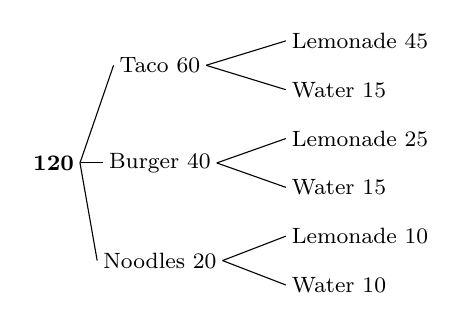
\begin{tikzpicture}[x=1cm, y=0.62cm, font=\footnotesize, inner sep=2pt]
        \node (r) at (0,0) {\textbf{120}};
        \node (a) at (1.35,2)  {Taco 60};
        \node (b) at (1.35,0)  {Burger 40};
        \node (c) at (1.35,-2) {Noodles 20};
        \draw (r.east) -- (a.west); \draw (r.east) -- (b.west); \draw (r.east) -- (c.west);
        \node[anchor=west] (a1) at (2.95,2.5)  {Lemonade 45};
        \node[anchor=west] (a2) at (2.95,1.5)  {Water 15};
        \node[anchor=west] (b1) at (2.95,0.5)  {Lemonade 25};
        \node[anchor=west] (b2) at (2.95,-0.5) {Water 15};
        \node[anchor=west] (c1) at (2.95,-1.5) {Lemonade 10};
        \node[anchor=west] (c2) at (2.95,-2.5) {Water 10};
        \draw (a.east) -- (a1.west); \draw (a.east) -- (a2.west);
        \draw (b.east) -- (b1.west); \draw (b.east) -- (b2.west);
        \draw (c.east) -- (c1.west); \draw (c.east) -- (c2.west);
      \end{tikzpicture}
    \end{column}
    \begin{column}{0.46\textwidth}
      \small\renewcommand{\arraystretch}{1.25}
      \begin{tabular}{@{} l c c c @{}}
      \hline
      & \textbf{Lem.} & \textbf{Water} & \textbf{Total} \\
      \hline
      Taco & 45 & 15 & 60 \\
      Burger & 25 & 15 & 40 \\
      Noodles & 10 & 10 & 20 \\
      \textbf{Total} & 80 & 40 & 120 \\
      \hline
      \end{tabular}
    \end{column}
  \end{columns}
  \vspace{6pt}
  \begin{itemize}\setlength{\itemsep}{3pt}
    \item $P(\text{burger and water}) = \frac{15}{120} = \frac18$ \quad (read the end of one path).
    \item $P(\text{lemonade}) = \frac{80}{120} = \frac23$ \quad (the table's column total is one number).
  \end{itemize}
\end{frame}

% ── ROW 4: REGIONS ───────────────────────────────────────────────────────────
\begin{frame}[t, plain]
  \ceruleanheader{Every region has a name}
  \sectionlabel{notes row 4 $\cdot$ Venn Diagram $\cdot$ problems 7--8}
  \begin{columns}[c]
    \begin{column}{0.54\textwidth}
      \venn{Taco\\(18 in all)}{Lemonade\\(15 in all)}{\large 13}{\large 5}{\large 10}{\large 12}
    \end{column}
    \begin{column}{0.42\textwidth}
      \begin{itemize}\setlength{\itemsep}{4pt}
        \item \textbf{Intersection}: 5
        \item \textbf{Only} lemonade: 10
        \item \textbf{Neither}: 12
        \item \textbf{Union}: everything inside either circle
      \end{itemize}
    \end{column}
  \end{columns}
  \vspace{6pt}
  \begin{block}{Problem 8: Reese says $P(\text{only lemonade}) = \frac{15}{40}$}
    The 15 is the \redink{whole circle}, overlap included. Only lemonade is $\frac{10}{40} = \frac14$.
  \end{block}
\end{frame}

% ── ROW 4: THE CRUX ──────────────────────────────────────────────────────────
\begin{frame}[t, plain]
  \ceruleanheader{Vote again: is Dani's 33 right?}
  \sectionlabel[redacc]{notes row 4 $\cdot$ problems 9--10 $\cdot$ the whole point of today}
  \begin{columns}[c]
    \begin{column}{0.54\textwidth}
      \venn{Taco\\(18 in all)}{Lemonade\\(15 in all)}{\large 13}{\large\textcolor{redacc}{\textbf{5}}}{\large 10}{\large 12}
    \end{column}
    \begin{column}{0.42\textwidth}
      \begin{itemize}\setlength{\itemsep}{4pt}
        \item Dani: $18 + 15 =$ \redink{33}
        \item Region by region: $13 + 5 + 10 =$ \redink{28}
        \item $P(\text{taco or lemonade}) = \frac{28}{40} = \frac{7}{10}$
        \item Check: $1 - \frac{12}{40} = \frac{28}{40}$
      \end{itemize}
    \end{column}
  \end{columns}
  \vspace{6pt}
  \begin{block}{Adding the two circle totals counts the overlap twice}
    To count ``or,'' add the regions inside the circles, each one once.
  \end{block}
\end{frame}

% ── WE DO — a LIVE surface: task and data only, no answers ───────────────────
\begin{frame}[t, plain]
  \ceruleanheader{Guided Practice: The Team Roster}
  \sectionlabel[goldacc]{We do $\cdot$ problems 11--14 $\cdot$ you hold the pen}
  \begin{columns}[c]
    \begin{column}{0.48\textwidth}
      \venn{Soccer\\(15 in all)}{Basketball\\(9 in all)}{?}{4}{?}{?}\\[3pt]
      {\small 30 athletes on the roster}
    \end{column}
    \begin{column}{0.5\textwidth}
      \small
      \begin{itemize}\setlength{\itemsep}{3pt}
        \item[11.] Fill in the four regions.
        \item[12.] $P(\text{only basketball})$ and $P(\text{neither sport})$.
        \item[13.] Coach: ``$15 + 9 = 24$ play soccer or basketball.'' Find
              $P(\text{soccer or basketball})$. Is Coach right?
        \item[14.] Soccer and basketball: mutually exclusive? ``Soccer or basketball'' and
              ``neither'': complementary?
      \end{itemize}
    \end{column}
  \end{columns}
\end{frame}

% ── DEBRIEF ──────────────────────────────────────────────────────────────────
\begin{frame}[t, plain]
  \ceruleanheader{Debrief: each region once}
  \sectionlabel{5 minutes $\cdot$ pens down, papers up --- we say these aloud}
  \vspace{4pt}
  \begin{enumerate}\setlength{\itemsep}{5pt}
    \item Problem 13: $11 + 4 + 5 = 20$, not 24. Say the sentence --- \emph{adding the circle
          totals counts the overlap twice.}
  \end{enumerate}
  \vspace{6pt}
  \begin{block}{Cold check --- hands down, thirty seconds}
    32 students: \textbf{16} are in band, \textbf{10} in choir, and \textbf{6} in both.
    \textbf{How many are in band or choir? How many are in only choir?}
  \end{block}
\end{frame}

% ── YOU DO — the homework is the individual practice, assigned today ─────────
\begin{frame}[t, plain]
  \ceruleanheader{You do: the homework}
  \sectionlabel[goldacc]{Assigned today $\cdot$ on your own, outside class $\cdot$ due after two study halls}
  \begin{itemize}\setlength{\itemsep}{5pt}
    \item \textbf{A bookstore loyalty program} --- a rewards wheel and a members survey.
    \item A probability, a prediction and what it means, and a complement.
    \item A Venn diagram: the whole circle against the ``only'' region.
    \item A claim that adds two circle totals, and a two-way table from Lesson 3.1.
  \end{itemize}
  \begin{block}{DeltaMath (theoretical probability, or / and counts, two-way tables) + turn in packet items 1, 2, 4, 5. Scored 1 to 5, due at the start of the first class after two study halls.}
    Do item 5 first if you are short on time. Your notes' rows 2 and 4 and the \emph{Keep in
    Mind} box are your reference.
  \end{block}
\end{frame}

% ── CLOSE ────────────────────────────────────────────────────────────────────
{
\setbeamercolor{background canvas}{bg=cerulean}
\begin{frame}[plain]
  \vspace{1.5cm}\hspace{0.8cm}%
  \begin{minipage}{0.86\textwidth}
    {\color{goldacc}\bfseries\small BEFORE YOU GO}\\[0.7cm]
    {\color{white}\bfseries\Large A circle's total includes the overlap. To count ``or,'' add
    each region once.}\\[0.9cm]
    {\color{frostmid}\small Next: Lesson 3.3, Addition and Multiplication Rules.}
  \end{minipage}
\end{frame}
}

\end{document}
